\documentclass[12pt,letterpaper]{report}

% Preamble for pmath347_notes.tex

\usepackage[dvipsnames, table]{xcolor}

\usepackage{amsmath}
\usepackage{amssymb}
\usepackage{amsthm}
\usepackage{changepage}
\usepackage{enumitem}
\usepackage{fancyhdr}
\usepackage{forest}
\usepackage{fullpage}
\usepackage{geometry}
\usepackage{graphicx}
%\usepackage{bbold}
\usepackage{mathrsfs}
\usepackage{mathtools}
\usepackage{multicol}
\usepackage{multirow}
\usepackage{parskip}
\usepackage[notmath]{sansmathfonts}
\usepackage{stmaryrd}
\usepackage{tabularx}
\usepackage[most]{tcolorbox}
\usepackage{tikz}
\usepackage{titlesec}
\usepackage{titletoc}
\usepackage[titles]{tocloft}
\usepackage[normalem]{ulem}

\usepackage[
  pdftitle={PMATH 347 Notes},
  pdfsubject={University of Waterloo, Spring 2021 (William Slofstra)},
  pdfauthor={Marco Yang <kc4yang@uwaterloo.ca>},
  colorlinks=true,
  linkcolor=blue
]{hyperref}
\usepackage[nameinlink]{cleveref}

\usetikzlibrary{arrows.meta}

%% Layout

\graphicspath{{./img/}}

% Margins
\geometry{
  margin=1in,
  headheight=1ex + \baselineskip,
  headsep=\baselineskip
}

% Header/footer
\pagestyle{fancy}
\fancyhf{}
\renewcommand{\headrulewidth}{0pt}
\renewcommand{\sectionmark}[1]{\markboth{\thesection\hspace{1.5ex}{#1}}{}}
\fancyhead[L]{\color{black!50} \small \sffamily PMATH 347}
\fancyhead[R]{\color{black!50} \small \sffamily \leftmark}
\fancyfoot[C]{\color{black!50} \small \sffamily \thepage}

% Chapters
\counterwithout*{section}{chapter} % Don't reset section number in new chapter
\titleformat{\chapter}
  {\huge \sffamily \bfseries \centering} % Format
  {Week \thechapter:} % Label
  {1ex} % Sep
  {} % Before
\titlecontents{chapter}
  [0em] % Left spacing
  {\vspace{\baselineskip}} % Above
  {\large \bfseries \contentslabel{2em}} % Numbered format
  {\large \bfseries} % Numberless format
  {\hfill} % Filler page format
  [\vspace{\baselineskip}] % Below

% Sections
\renewcommand{\thesection}{\arabic{section}}
\newcommand{\sectionbreak}{\clearpage\phantomsection}
\titleformat{\section}
  {\Large \sffamily \bfseries} % Format
  {\thesection:} % Label
  {1ex} % Sep
  {} % Before
\titlecontents{section}
  [3em] % Left spacing
  {} % Above
  {\bfseries \contentslabel{2em}} % Numbered format
  {} % Numberless format
  {\titlerule*{$\cdot$}\contentspage} % Filler page format
  [] % Below

% Subsections
\titleformat{\subsection}
  {\large \sffamily \bfseries} % Format
  {} % Label
  {0pt} % Sep
  {} % Before
\titlecontents{subsection}
  [3em] % Left spacing
  {} % Above
  {} % Numbered format
  {} % Numberless format
  {\hfill} % Filler page format
  [] % Below

%% Commands

% New week
\newcommand{\week}[1]{
  \chapter{#1}
  \thispagestyle{empty}
  \pagebreak
}

% Environments
\newtcbtheorem[no counter]
  {thm} % environment name
  {Theorem} % display name
  { % options
    colback=blue!10,
    colframe=blue!10,
    colbacktitle=blue!10,
    coltitle=blue!60!black,
    fonttitle=\sffamily\bfseries,
    sharp corners,
    boxsep=1ex,
    toptitle=1ex,
    before skip=\baselineskip,
    after skip=\baselineskip,
    separator sign={~---},
    label type=thm
  }
  {thm} % label prefix
\crefname{thm}{Theorem}{Theorems}

\newtcbtheorem[no counter]
  {lem} % environment name
  {Lemma} % display name
  { % options
    colback=blue!10,
    colframe=blue!10,
    colbacktitle=blue!10,
    coltitle=blue!60!black,
    fonttitle=\sffamily\bfseries,
    sharp corners,
    boxsep=1ex,
    toptitle=1ex,
    before skip=\baselineskip,
    after skip=\baselineskip,
    separator sign={~---},
    label type=lem
  }
  {lem} % label prefix
\crefname{lem}{Lemma}{Lemmas}

\newtcbtheorem[no counter]
  {cor} % environment name
  {Corollary} % display name
  { % options
    colback=blue!10,
    colframe=blue!10,
    colbacktitle=blue!10,
    coltitle=blue!60!black,
    fonttitle=\sffamily\bfseries,
    sharp corners,
    boxsep=1ex,
    toptitle=1ex,
    before skip=\baselineskip,
    after skip=\baselineskip,
    separator sign={~---},
    label type={cor}
  }
  {cor} % label prefix
\crefname{cor}{Corollary}{Corollaries}

\newtcbtheorem[no counter]
  {prop} % environment name
  {Proposition} % display name
  { % options
    colback=blue!10,
    colframe=blue!10,
    colbacktitle=blue!10,
    coltitle=blue!60!black,
    fonttitle=\sffamily\bfseries,
    sharp corners,
    boxsep=1ex,
    toptitle=1ex,
    before skip=\baselineskip,
    after skip=\baselineskip,
    separator sign={~---},
    label type={prop}
  }
  {prop} % label prefix
\crefname{prop}{Proposition}{Propositions}

\newtcbtheorem[no counter]
  {exer} % environment name
  {Exercise} % display name
  { % options
    colback=red!10,
    colframe=red!10,
    colbacktitle=red!10,
    coltitle=red!60!black,
    fonttitle=\sffamily\bfseries,
    sharp corners,
    boxsep=1ex,
    toptitle=1ex,
    before skip=\baselineskip,
    after skip=\baselineskip,
    separator sign={~---},
    label type={exer}
  }
  {exer} % label prefix
\crefname{exer}{Exercise}{Exercises}

\newtcbtheorem[no counter]
  {defn} % environment name
  {Definition} % display name
  { % options
    parbox=false,
    nameref/.style={},
    colback=green!10,
    colframe=green!10,
    colbacktitle=green!10,
    coltitle=green!60!black,
    fonttitle=\sffamily\bfseries,
    sharp corners,
    boxsep=1ex,
    toptitle=1ex,
    before skip=\baselineskip,
    after skip=\baselineskip,
    separator sign={~---},
    label type={defn}
  }
  {defn} % label prefix
\crefname{defn}{Definition}{Definitions}

\newtcbtheorem[no counter]
  {axiom} % environment name
  {Axiom} % display name
  { % options
    colback=blue!10,
    colframe=blue!10,
    colbacktitle=blue!10,
    coltitle=blue!60!black,
    fonttitle=\sffamily\bfseries,
    sharp corners,
    boxsep=1ex,
    toptitle=1ex,
    before skip=\baselineskip,
    after skip=\baselineskip,
    separator sign={~---},
    label type={prop}
  }
  {axiom} % label prefix
\crefname{axiom}{Axiom}{Axiom}

\newtcolorbox{ex}[1][Example]{
  enhanced,
  parbox=false,
  sharp corners,
  breakable,
  boxrule=0pt,
  left=1ex + 2mm + 4pt,
  right=0pt,
  bottom=0pt,
  frame hidden,
  title={#1},
  fonttitle=\sffamily\bfseries,
  colback=white,
  coltitle=red!60!black,
  colbacktitle=white,
  borderline west={4pt}{0pt}{red!60!black},
  before skip=\baselineskip,
  after skip=\baselineskip
}

\makeatletter
\newenvironment{proofb}{%
  \par
  \pushQED{\qed}
  \normalfont \topsep0\p@\@plus6\p@\relax
  \trivlist
  \item[]\ignorespaces
}{%
  \popQED\endtrivlist\@endpefalse
}
\makeatother

\newenvironment{thmproof}[1][Proof.]{
  \begin{tcolorbox}[
    enhanced,
    breakable,
    parbox=false,
    sharp corners,
    boxrule=0pt,
    left=1ex + 2mm + 4pt,
    right=0pt,
    bottom=0pt,
    frame hidden,
    title={#1},
    fonttitle=\sffamily\itshape,
    colback=white,
    coltitle=blue!60!black,
    colbacktitle=white,
    borderline west={4pt}{0pt}{blue!60!black},
    before skip=\baselineskip,
    after skip=\baselineskip
  ]
  \begin{proofb}
}{
  \end{proofb}
  \end{tcolorbox}
}

\newenvironment{exerproof}[1][Proof.]{
  \begin{tcolorbox}[
    enhanced,
    breakable,
    parbox=false,
    sharp corners,
    boxrule=0pt,
    left=1ex + 2mm + 4pt,
    right=0pt,
    bottom=0pt,
    frame hidden,
    title={#1},
    fonttitle=\sffamily\itshape,
    colback=white,
    coltitle=red!60!black,
    colbacktitle=white,
    borderline west={4pt}{0pt}{red!60!black},
    before skip=\baselineskip,
    after skip=\baselineskip
  ]
  \begin{proofb}
}{
  \end{proofb}
  \end{tcolorbox}
}

% Emphasis
\newcommand{\hldef}[1]{\textcolor{green!60!black}{\textbf{#1}}}

% Circled numbers
\newcommand*\circled[1]{
  \tikz[baseline=(char.base)]{
    \node[shape=circle, draw, inner sep=2pt] (char) {\footnotesize #1};
  }
}

% Enum with circled numbers
\newenvironment{enumcase}[1][]{
  \begin{enumerate}[label=\protect\circled{\arabic*}, #1]
}{
  \end{enumerate}
}

%% Math commands

% Useful delimiters: abs
\DeclarePairedDelimiter\abs{\lvert}{\rvert}
\DeclarePairedDelimiter\norm{\lVert}{\rVert}
\DeclarePairedDelimiter\ceil{\lceil}{\rceil}
\DeclarePairedDelimiter\floor{\lfloor}{\rfloor}
\DeclarePairedDelimiter\ang{\langle}{\rangle}

% Operators and such
\DeclareMathOperator{\Id}{Id}
\DeclareMathOperator{\GL}{GL}
\DeclareMathOperator{\PGL}{PGL}
\DeclareMathOperator{\SL}{SL}
\DeclareMathOperator{\Fun}{Fun}
\DeclareMathOperator{\Hom}{Hom}
\DeclareMathOperator{\Sub}{Sub}
\DeclareMathOperator{\supp}{supp}
\let\Im\relax
\DeclareMathOperator{\Im}{Im}
\DeclareMathOperator{\Conj}{Conj}
\DeclareMathOperator{\Span}{Span}
\DeclareMathOperator{\charc}{char}
\DeclareMathOperator{\ev}{ev}
\DeclareMathOperator{\lcm}{lcm}

% Macros
\newcommand{\N}{\mathbb{N}}
\newcommand{\Z}{\mathbb{Z}}
\newcommand{\Q}{\mathbb{Q}}
\newcommand{\R}{\mathbb{R}}
\newcommand{\C}{\mathbb{C}}
\newcommand{\K}{\mathbb{K}}
\newcommand{\Zmod}[1]{\mathbb{Z}/{#1}\mathbb{Z}}
\newcommand{\orbit}{\mathcal{O}}
\newcommand{\ideal}{\mathcal{I}}


%---------------
\begin{document}
%--------------

%%%%% Title
\title{
  \Huge
  \textbf{PMATH 347: Groups and Rings} \\[\baselineskip]
  \large
  University of Waterloo \\
  William Slofstra \\
  Spring 2021
}
\author{Marco Yang}
\date{Last updated: \today}

{
  \sffamily
  \maketitle
}
\thispagestyle{empty}

%%%%% Table of contents
\pagebreak
\pagenumbering{roman}
\setcounter{page}{2}

{
  \sffamily
  \tableofcontents{\markboth{\contentsname}{}}
}

%%%%% Lectures
\pagebreak
\pagenumbering{arabic}

\week{Groups}

%%%%% Lec 1
\section{Binary operations and definition of a group}

\subsection{Binary operations}

\begin{defn}{binary operation}{binop}
  A \hldef{binary operation} on a set $X$ is a function $b \colon X \times X \to X$.
\end{defn}

Notation:
\begin{itemize}
  \item
  We can use any letter ($b$, $m$) or symbol ($+$, $\cdot$).
  \item
  We can use function notation (typically for symbols)
  \[ b \colon X \times X \to X : (x, y) \mapsto b(x, y) \]
  or inline notation (typically for letters)
  \[ + \colon \mathbb{N} \times \mathbb{N} \to \mathbb{N} : (x, y) \mapsto x + y. \]
  \item
  Some symbols: $a + b$, $a \times b$, $a \cdot b$, $a \circ b$, $a \oplus b$, $a \otimes b$,
  $a \odot b$, $a \diamond b$, $a * b$, $a \bullet b$, $a \boxplus b$, $a \boxtimes b$.
  \item
  If not ambiguous, can drop the symbol:
  \[ X \times X \to X : (a, b) \mapsto ab. \]
\end{itemize}

\begin{ex}
  \begin{itemize}
    \item
    Addition $+$ is a binary operation on $\mathbb{N}$, but subtraction $-$ is not since $a - b$ is
    not necessarily in $\mathbb{N}$.
    \item
    Subtraction is a binary operation on $\mathbb{Z}$, \emph{i.e.}, it defines a function
    $- \colon \mathbb{Z} \times \mathbb{Z} \to \mathbb{Z}$.
    \item
    If $(V, +, \cdot)$ is a vector space over a field $\mathbb{K}$, then $+$ is a binary operation
    on $V$, but $\cdot$ is not since $\cdot$ is a function $\mathbb{K} \times V \to V$.
  \end{itemize}
\end{ex}

\begin{defn}{$k$-ary operation}{karyop}
  A \hldef{$k$-ary operation} on a set $X$ is a function
  \[
    \underbrace{X \times X \times \cdots \times X}_{k \text{ times}} \to X.
  \]
  A $1$-ary operation is called a \hldef{unary operation}.
\end{defn}

\begin{ex}
  \begin{itemize}
    \item
    Negation $\mathbb{Z} \to \mathbb{Z} : x \mapsto -x$ is a unary operation.
    \item
    Taking the multiplicative inverse $x \mapsto 1/x$ is not a unary operation on $\mathbb{Q}$,
    since $1/0$ is not defined, but it is a unary operation on
    \[ \mathbb{Q}^\times := \{ a \in \mathbb{Q} : a \neq 0 \}. \]
  \end{itemize}
\end{ex}

\pagebreak
\subsection{Associative operations}

\begin{defn}{associative}{associative}
  A binary operation $\boxtimes \colon X \times X \to X$ is \hldef{associative} if
  \[
    a \boxtimes (b \boxtimes c) = (a \boxtimes b) \boxtimes c
  \]
  for all $a, b, c \in X$.
\end{defn}

Many operations mentioned so far are associative:
\begin{itemize}
  \item
  Addition and multiplication for $\mathbb{N}$, $\mathbb{Z}$, $\mathbb{Q}$, $\mathbb{R}$,
  $\mathbb{C}$, polynomials, and functions;
  \item
  Vector addition, matrix addition and multiplication;
  \item
  Modular addition and multiplication on $\mathbb{Z} / n\mathbb{Z}$;
  \item
  Function composition (homework).
\end{itemize}

Subtraction and division are not associative:
\[
  10 - (5 - 1) = 6 \neq 4 = (10 - 5) - 1.
\]
Subtraction is adding negative numbers; similarly for division.
So we aren't as interested in subtraction and division, thus we can focus on associative operations.

A \hldef{bracketing} of a sequence $a_1, \ldots, a_n \in X$ is a way of inserting brackets into
$a_1 \boxtimes \cdots \boxtimes a_n$ so that the expression can be evaluated (with binary steps).

\begin{ex}
  Bracketings of $a_1, \ldots, a_4$ are:
  \begin{itemize}
    \item $a_1 \boxtimes (a_2 \boxtimes (a_3 \boxtimes a_4))$
    \item $a_1 \boxtimes ((a_2 \boxtimes a_3) \boxtimes a_4)$
    \item $(a_1 \boxtimes a_2) \boxtimes (a_3 \boxtimes a_4)$
    \item $(a_1 \boxtimes (a_2 \boxtimes a_3)) \boxtimes a_4$
    \item $((a_1 \boxtimes a_2) \boxtimes a_3) \boxtimes a_4$
  \end{itemize}
\end{ex}

\begin{prop}{}{}
  A binary operation $\boxtimes \colon X \times X \to X$ is associative if and only if for all
  finite sequences $a_1, \ldots, a_n \in X$ with $n \geq 1$, every bracketing of $a_1, \ldots, a_n$
  evaluates to the same element of $X$.
\end{prop}

Meaning if $\boxtimes$ is associative, then the notation $a_1 \boxtimes \cdots \boxtimes a_n$ is
unambiguous.

\begin{thmproof}
  \begin{itemize}[leftmargin=4em]
    \item[($\impliedby$)]
    The two bracketings $a \boxtimes (b \boxtimes c)$ and $(a \boxtimes b) \boxtimes c$ of $a, b, c$
    evaluate to the same element of $X$ for all sequences of length 3.
    So $\boxtimes$ is associative by definition.

    \item[($\implies$)]
    By induction.
    Base cases are $n = 1, 2, 3$.
    For $n = 1, 2$, there is only one bracketing.
    For $n = 3$, follows from the definition of associativity.

    Suppose the proposition is true for all sequences of length $1 \leq k < n$.

    Let $w$ be a bracketing of $a_1, \ldots, a_n$.
    Then $w = w_1 \boxtimes w_2$ where $w_1$ is a bracketing of $a_1, \ldots, a_k$ and $w_2$ is a
    bracketing of $a_{k + 1}, \ldots, a_n$ for some $k < n$.
    By induction,
    \begin{align*}
      w_1 &= (\cdots ((a_1 \boxtimes a_2) \boxtimes a_3) \cdots \boxtimes a_k) \\
      w_2 &= (a_{k + 1} \boxtimes \cdots (a_{n - 2} \boxtimes (a_{n - 1} \boxtimes a_n)) \cdots)
    \end{align*}
    So by repeatedly applying associativity,
    \begin{align*}
      w
      &= (\cdots ((a_1 \boxtimes a_2) \boxtimes a_3) \cdots \boxtimes a_k) \boxtimes
        (a_{k + 1} \boxtimes \cdots (a_{n - 1} \boxtimes a_n) \cdots) \\
      &= (\cdots (a_1 \boxtimes a_2) \cdots \boxtimes a_{k - 1}) \boxtimes
        (a_k \boxtimes (a_{k + 1} \boxtimes \cdots \boxtimes a_n) \cdots) \\
      &= \ldots \\
      &= (a_1 \boxtimes (a_2 \boxtimes \cdots (a_{n - 1} \boxtimes a_n)) \cdots)
    \end{align*}
  \end{itemize}
\end{thmproof}

\pagebreak
\subsection{Commutative (abelian) operations}

\begin{defn}{commutative (abelian)}{abelian}
  A binary operation $\boxtimes \colon X \times X \to X$ is \hldef{commutative} or \hldef{abelian}
  if $a \boxtimes b = b \boxtimes a$ for all $a, b \in X$.
\end{defn}

Many familiar operations are commutative:
\begin{itemize}
  \item
  Addition and multiplication on $\mathbb{N}$, $\mathbb{Z}$, $\mathbb{Q}$, $\mathbb{R}$,
  $\mathbb{C}$
  \item
  Vector and matrix addition
  \item
  Modular addition and multiplication on $\mathbb{Z} / n\mathbb{Z}$
\end{itemize}
The following operations are \textbf{not} commutative:
\begin{itemize}
  \item Subtraction and division: $3 - 1 \neq 1 - 3$
  \item Function composition
  \item Matrix multiplication
\end{itemize}

Note:
\begin{enumerate}
  \item Subtraction and division are not commutative or associative
  \item Function composition and matrix multiplication are not commutative, but are associative
\end{enumerate}
We won't study operations like (1), but we are interested in those like (2).

The first half of this course is group theory: single associative operation, not necessarily
commutative.

The second half of this course is ring theory: two associative operations, focus on the both
commutative case.

\pagebreak
\subsection{Identities}

\begin{defn}{identity}{identity}
  Let $\boxtimes$ be a binary operation on a set $X$.
  An element $e \in X$ is an \hldef{identity} for $\boxtimes$ if
  \[ e \boxtimes x = x \boxtimes e = x \]
  for all $x \in X$.
\end{defn}

\begin{ex}
  \begin{itemize}
    \item
    The zero element $0$ of $\mathbb{Z}$ is an identity for $+$, since $0 + x = x + 0 = x$ for all
    $x \in \mathbb{Z}$.
    \item
    $1 \in \mathbb{Q}$ is an identity for $\cdot$, since $1 \cdot x = x \cdot 1 = x$ for all
    $x \in \mathbb{Q}$.
    \item
    $0 \in \mathbb{Q}$ is not an identity for $\cdot$, since $0 \cdot x = 0 \neq x$ for all
    $x \in \mathbb{Q}$.
  \end{itemize}
\end{ex}

\begin{lem}{}{}
  If $e, e' \in X$ are both identities for $\boxtimes$, then $e = e'$.
\end{lem}

\begin{thmproof}
  $e = e \boxtimes e' = e'$.
\end{thmproof}

\pagebreak
\subsection{Inverses}

\begin{defn}{inverse}{inverse}
  Let $\boxtimes$ be a binary operation on $X$ with an identity element $e$.
  An element $y$ is a \hldef{left inverse} for $x$ (with respect to $\boxtimes$) if
  $y \boxtimes x = e$, a \hldef{right inverse} if $x \boxtimes y = e$, and an \hldef{inverse} if
  $x \boxtimes y = y \boxtimes x = e$.
\end{defn}

\begin{ex}
  \begin{itemize}
    \item
    $-n$ is an inverse for $n \in \mathbb{Z}$ with respect to $+$, since $n + (-n) = (-n) + n = 0$.
    \item
    $n \in \mathbb{Z}$ does not have an inverse with respect to $\cdot$ unless $n = \pm 1$.
    \item
    If $x \in \mathbb{Q}$ is non-zero, then $1/x$ is an inverse of $x$ with respect to $\cdot$.
    The element $0$ does not have an inverse, since there is no element $y$ with $0 \cdot y = 1$.
  \end{itemize}
\end{ex}

\begin{lem}{}{}
  Let $\boxtimes$ be an associative binary operation with an identity $e$.
  If $y_L$ and $y_R$ are left and right inverses of $x$ respectively, then $y_L = y_R$.
\end{lem}

\begin{thmproof}
  $y_L = y_L \boxtimes e = y_L \boxtimes (x \boxtimes y_R) = (y_L \boxtimes x) \boxtimes y_R =
    e \boxtimes y_R = y_R$.
\end{thmproof}

Corollaries:
\begin{itemize}
  \item If $x$ has both a left and a right inverse, then $x$ has an inverse.
  \item Inverses are unique: if $y$ and $y'$ are both inverses of $x$, then $y = y'$.
\end{itemize}

An element $a$ is \hldef{invertible} if it has an inverse, in which case the inverse is denoted by
$a^{-1}$.

\begin{exer}{}{}
  Show it is possible to have a left (resp. right) inverse, but not be invertible.
  Also show left and right inverses are not necessarily unique (unless an element has both).
\end{exer}

\pagebreak
\subsection{Properties of inverses}

\begin{lem}{}{}
  \begin{enumerate}
    \item
    If $\boxtimes$ has an identity $e$, then $e$ is invertible, and $e^{-1} = e$.
    \item
    If $a$ is invertible, then so is $a^{-1}$, and $(a^{-1})^{-1} = a$.
    \item
    If $\boxtimes$ is associative, and $a$ and $b$ are invertible, then so is $a \boxtimes b$, and
    $(a \boxtimes b)^{-1} = b^{-1} \boxtimes a^{-1}$.
  \end{enumerate}
\end{lem}

\begin{thmproof}
  \begin{enumerate}
    \item
    $e \boxtimes e = e$.
    \item
    $a \boxtimes a^{-1} = a^{-1} \boxtimes a = e$, so $a$ is an inverse to $a^{-1}$.
    \item
    $(a \boxtimes b) \boxtimes (b^{-1} \boxtimes a^{-1}) =
      a \boxtimes (b \boxtimes b^{-1}) \boxtimes a^{-1} = a \boxtimes e \boxtimes a^{-1} =
      a \boxtimes a^{-1} = e$,
    and similarly $(b^{-1} \boxtimes a^{-1}) \boxtimes (a \boxtimes b) = e$.
  \end{enumerate}
\end{thmproof}

\pagebreak
\subsection{Inverses and solving equations}

\begin{prop}{}{}
  Let $\boxtimes$ be an associative binary operation on $X$ with an identity $e$, and let $x$ and
  $y$ be variables taking values in $X$.

  An element $a \in X$ is invertible if and only if the equations $a \boxtimes x = b$ and
  $y \boxtimes a = b$ have unique solutions for all $b \in X$.
\end{prop}

\begin{thmproof}
  \begin{itemize}[leftmargin=4em]
    \item[($\impliedby$)]
    A solution to $a \boxtimes x = e$ is a right inverse of $a$, and a solution to
    $y \boxtimes a = b$ is a left inverse.
    Since both solutions exist, $a$ has an inverse.
    \item[($\implies$)]
    Suppose $a$ is invertible.
    Then
    \[ a \boxtimes (a^{-1} \boxtimes b) = (a \boxtimes a^{-1}) \boxtimes b = e \boxtimes b = b \]
    so $a^{-1} \boxtimes b$ is a solution to $a \boxtimes x = b$.

    If $x_0$ is a solution to $a \boxtimes x = b$, then
    \[
      a^{-1} \boxtimes b = a^{-1} \boxtimes (a \boxtimes x_0) = (a^{-1} \boxtimes a) \boxtimes x_0
        = e \boxtimes x_0 = x_0
    \]
    so $a^{-1} \boxtimes b$ is the unique solution to $a \boxtimes x = b$.

    Similarly, $b \boxtimes a^{-1}$ is the unique solution to $y \boxtimes a = b$.
  \end{itemize}
\end{thmproof}

\pagebreak
\subsection{Left and right cancellation property}

\begin{prop}{}{}
  Let $\boxtimes$ be an associative binary operation and let $a \in X$.
  Then:
  \begin{enumerate}
    \item If $a$ has a left inverse and $a \boxtimes u = a \boxtimes v$, then $u = v$.
    \item If $a$ has a right inverse and $u \boxtimes a = v \boxtimes a$, then $u = v$.
  \end{enumerate}
\end{prop}

\begin{thmproof}
  \begin{enumerate}
    \item $u = a_L \boxtimes a \boxtimes u = a_L \boxtimes a \boxtimes v = v$.
    \item Similar.
  \end{enumerate}
\end{thmproof}

(1) and (2) also hold for $n \in \mathbb{Z}$ with respect to $\cdot$ if $n \neq 0$, even though $n$
is not invertible for $n \neq \pm 1$.

\pagebreak
\subsection{Groups}

\begin{defn}{group}{group}
  A \hldef{group} is a pair $(G, \boxtimes)$ where
  \begin{enumerate}
    \item $G$ is a set, and
    \item $\boxtimes$ is an associative binary operation on $G$ such that
    \begin{enumerate}
      \item $\boxtimes$ has an identity $e$, and
      \item every element $g \in G$ is invertible with respect to $\boxtimes$.
    \end{enumerate}
  \end{enumerate}

  A group is \hldef{abelian} (or \hldef{commutative}) if $\boxtimes$ is abelian.

  A group is \hldef{finite} if $G$ is a finite set.
  The \hldef{order} of $G$ is the number of elements in $G$ if $G$ is finite, or $+\infty$ if $G$ is
  infinite.

  The order of $G$ is denoted by $\abs{G}$.
\end{defn}

Terminology:
\begin{itemize}
  \item
  Usually we refer to $(G, \boxtimes)$ simply as $G$, and just assume the operation is given.
  (Note: we still need to clearly specify the operation for each group we work with.)
  \item
  It's cumbersome to write $\boxtimes$, so usually we use one of the following options:
  \begin{itemize}
    \item Use $\cdot$ as the standard symbol: $g \cdot h$ is the product of $g, h \in G$.
    \item Drop the symbol entirely: $gh$ is the product of $g, h \in G$.
  \end{itemize}
  \item
  The identity of $G$ is denoted by $e$ (or $e_G$ for clarity).
  Also used are $1$ and $1_G$.
  \item
  $g^{-1}$ is defined for all $g \in G$.
  The function $G \to G : g \mapsto g^{-1}$ can be regarded as a unary operation on $G$.
  \item
  Consider $\iota \colon G \to G : g \mapsto g^{-1}$.
  Since $(g^{-1})^{-1} = g$, $\iota \circ \iota = \Id_G$, the identity map $G \to G$.
  In particular, $\iota$ is a bijection (injective and surjective).
  \item
  If $g \in G$, then
  \[ g^n := \underbrace{g \cdots g}_{n \text{ times}} \]
  and
  \[ g^{-n} := (g^{-1})^n = (g^n)^{-1} \]
  where $g^0 := e$.
  Exercise: if $m, n \in \mathbb{Z}$, then $(g^n)^m = g^{mn}$.
  \item
  If $g, h \in G$, then
  \[ (gh)^n = gh \cdots gh, \]
  which is not necessarily the same as $g^n h^n$ if $G$ is not abelian.
\end{itemize}

\begin{ex}
  \begin{itemize}
    \item
    $\mathbb{Z}$, $\mathbb{Q}$, $\mathbb{R}$, $\mathbb{C}$ are all (abelian) groups under operation
    $+$.
    The identity is $0$ and the inverse of $n$ is $-n$.
    These groups have infinite order.
    \item
    $\mathbb{Z} / n\mathbb{Z}$ is also a group under $+$ (and also abelian).
    The identity is $0 = [0]$ and the inverse of $[m]$ is $-[m] = [-m]$.
    This group is finite with order $\abs{\mathbb{Z} / n\mathbb{Z}} = n$.
    \item
    If $(V, +, \cdot)$ is a vector space, then $(V, +)$ is a group.
    The identity is $0$ and the inverse of $v$ is $-v$.
    \item
    $\mathbb{Z}$ is not a group with respect to $\cdot$, since most elements do not have an inverse.
    \item
    $\mathbb{Q}$ is also not a group with respect to $\cdot$, since $0$ does not have an inverse.
    \item
    $\mathbb{Q}^\times$ is a group with respect to $\cdot$.
    \item
    Every group has to contain at least one element, the identity.
    So the simplest possible group is ${1}$ with operation $1 \cdot 1 = 1$.
    This is the \hldef{trivial group}.
  \end{itemize}
\end{ex}

\pagebreak
\subsection{A non-abelian example}

All the previous examples are abelian.

Let $\GL_n(\mathbb{K})$ denote the invertible $n \times n$ matrices over a field $\mathbb{K}$.

\begin{prop}{}{}
  $\GL_n(\mathbb{K})$ is a group under matrix multiplication (called the
  \hldef{general linear group}).
  For $n \geq 2$, $\GL_n(\mathbb{K})$ is non-abelian.
\end{prop}

\begin{thmproof}
  If $A$ and $B$ are invertible matrices, then $AB$ is also invertible, so matrix multiplication is
  an associative binary operation on $\GL_n(\mathbb{K})$.
  The identity matrix is an identity and every element has an inverse by definition, so
  $\GL_n(\mathbb{K})$ is a group.

  Exercise: find matrices $A, B$ such that $AB \neq BA$.
\end{thmproof}

\pagebreak
\subsection{Additive notation}

Standard notation for a group operation is $gh$.
This is called \hldef{multiplicative notation}.

For groups like $(\mathbb{Z}, +)$, it is confusing to write $mn$ instead of $m + n$ since $mn$
already has another meaning.

For abelian groups $G$, we can also use \hldef{additive notation}.
In additive notation, we write the group operation as $g + h$.
The identity is denoted by $0$ or $0_G$.
Inverses are denoted by $-g$.

Writing $g^n$ in additive notation gives
\[ \underbrace{g + \cdots + g}_{n \text{ times}} \]
so instead of $g^n$ we use $ng$.
Similarly $g^{-n}$ is $-ng$.

\begin{center}
  \renewcommand{\arraystretch}{1.2}
  \begin{tabular}{cc}
    Multiplicative notation & Additive notation \\
    \hline
    $g \cdot h$ or $gh$ & $g + h$ \\
    $e_G$ or $1_G$ & $0_G$ \\
    $g^{-1}$ & $-g$ \\
    $g^n$ & $ng$ \\
  \end{tabular}
\end{center}

For non-abelian groups we always use multiplicative notation.
For abelian groups, we can choose either.
Note the conventions may conflict, so we should be clear about which we choose.

For a group like $(\mathbb{Z}, +)$, we could use $mn$, but it is clearer to use $m + n$.

For a group like $(\mathbb{Q}^\times, \cdot)$, we could use $x + y$, but it is clearer to use
$x \cdot y$ or $xy$.

\pagebreak
\subsection{Multiplication table}

\begin{defn}{multiplication table}{multtable}
  The \hldef{multiplication table} of a group $G$ is a table with rows and columns indexed by the
  elements of $G$.
  The cell for row $g$ and column $h$ contains the product $gh$.
\end{defn}

The multiplication table contains the complete information of the group (even for infinite groups).

\begin{ex}
  For $\mathbb{Z} / 2\mathbb{Z}$:
  \[
    \begin{array}{c|cc}
      & 0 & 1 \\
      \hline
      0 & 0 & 1 \\
      1 & 1 & 0 \\
    \end{array}
  \]
\end{ex}

\pagebreak
\subsection{Order of elements}

\begin{defn}{order of a group element}{order_element}
  If $G$ is a group, then the order of $g \in G$ is
  \[ \abs{g} := \min\{ k \geq 1 : g^k = e_G \} \cup \{ +\infty \}. \]
\end{defn}

Easy properties:
\begin{itemize}
  \item $\abs{g} = 1$ if and only if $g = e_G$.
  \item If $g^n = 1$, then $g^{n - 1}g = gg^{n - 1} = g^n = 1$, so $g^{n - 1} = g^{-1}$.
  In particular, if $\abs{g} = n < \infty$, then $g^{-1} = g^{n - 1}$.
\end{itemize}

\begin{ex}
  We use additive notation for $\mathbb{Z} / n\mathbb{Z}$, so $g^n$ is written as $ng$ and $e = 0$.
  For this group, $k1 = 0$ if and only if $n \mid k$, so $\abs{1} = n$.
\end{ex}

\begin{lem}{}{}
  $g^n = e$ if and only if $g^{-n} = e$, so in particular, $\abs{g} = \abs{g^{-1}}$.
\end{lem}

\begin{thmproof}
  We have $g^{-n} = (g^n)^{-1}$.
  Since $g \mapsto g^{-1}$ is a bijection, $g^n = e$ if and only if $(g^n)^{-1} = e^{-1} = e$.

  But $g^{-n} = (g^{-1})^n$ also, so $\{ k \geq 1 : g^k = e \} = \{ k \geq 1 : (g^{-1})^k = e \}$
  which implies $\abs{g} = \abs{g^{-1}}$.
\end{thmproof}

%%%%% Lec 02
\section{Dihedral and permutation groups}

\subsection{Dihedral groups}

\begin{defn}{$n$-gon}{ngon}
  A regular polygon $P_n$ with $n \geq 3$ vertices is called an \hldef{$n$-gon}.
\end{defn}

Specifically: set $v_k = (\cos(2\pi k/n), \sin(2\pi k/n)) = e^{2\pi ik/n}$ and get an $n$-gon by
drawing a line segment from $v_k$ to $v_{k + 1}$ for all $0 \leq k \leq n$ (where $v_n := v_0$).

\begin{center}
  \begin{tabular}{
    >{\centering\arraybackslash}m{0.3\textwidth}
    >{\centering\arraybackslash}m{0.3\textwidth}
    >{\centering\arraybackslash}m{0.3\textwidth}
  }
    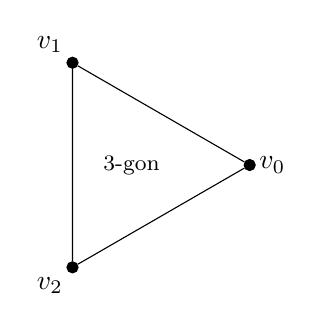
\begin{tikzpicture}[
      vtx/.style={
        circle, draw, fill=black,
        inner sep=0pt, minimum width=4pt
      }
    ]
      \foreach \ang/\x in {0/v0,120/v1,240/v2} {
        \node[vtx] (\x) at (\ang:1.5){};
      }
      \node[font=\footnotesize] at (0,0){$3$-gon};
      \node[right] at (v0){$v_0$};
      \node[above left] at (v1){$v_1$};
      \node[below left] at (v2){$v_2$};

      \draw (v0)--(v1)--(v2)--(v0);
    \end{tikzpicture}
    &
    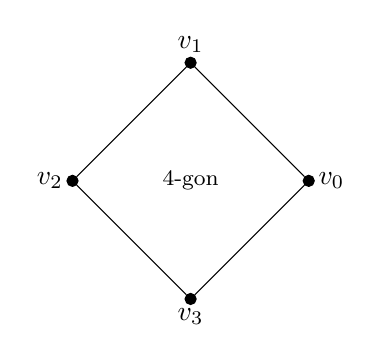
\begin{tikzpicture}[
      vtx/.style={
        circle, draw, fill=black,
        inner sep=0pt, minimum width=4pt
      }
    ]
      \foreach \ang/\x in {0/v0,90/v1,180/v2,270/v3} {
        \node[vtx] (\x) at (\ang:1.5){};
      }
      \node[font=\footnotesize] at (0,0){$4$-gon};
      \node[right] at (v0){$v_0$};
      \node[above] at (v1){$v_1$};
      \node[left] at (v2){$v_2$};
      \node[below] at (v3){$v_3$};

      \draw (v0)--(v1)--(v2)--(v3)--(v0);
    \end{tikzpicture}
    &
    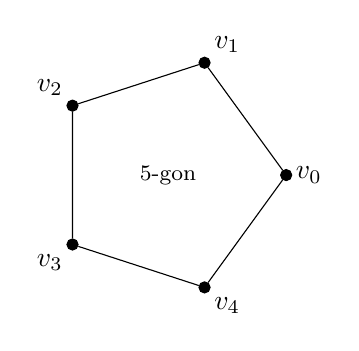
\begin{tikzpicture}[
      vtx/.style={
        circle, draw, fill=black,
        inner sep=0pt, minimum width=4pt
      }
    ]
      \foreach \ang/\x in {0/v0,72/v1,144/v2,216/v3,288/v4} {
        \node[vtx] (\x) at (\ang:1.5){};
      }
      \node[font=\footnotesize] at (0,0){$5$-gon};
      \node[right] at (v0){$v_0$};
      \node[above right] at (v1){$v_1$};
      \node[above left] at (v2){$v_2$};
      \node[below left] at (v3){$v_3$};
      \node[below right] at (v4){$v_4$};

      \draw (v0)--(v1)--(v2)--(v3)--(v4)--(v0);
    \end{tikzpicture}
    \\
  \end{tabular}
\end{center}

\begin{defn}{symmetry, dihedral group}{symmetry_dihedralgroup}
  A \hldef{symmetry} of the $n$-gon $P_n$ is an invertible linear transformation
  $T \in \GL_2(\mathbb{R})$ such that $T(P_n) = P_n$.

  The set of symmetries of $P_n$ is called the \hldef{dihedral group} and is denoted by $D_{2n}$
  (or $D_n$).
\end{defn}

(Think of matrices and linear transformations interchangeably.
Matrix multiplication = composition of transformations.)

\begin{prop}{}{}
  $D_{2n}$ is a group under composition.
\end{prop}

Proof later (key point: $S, T \in D_{2n} \implies ST \in D_{2n}$).

\begin{lem}{}{}
  Say $v_i$ and $v_j$ are adjacent in $P_n$ if they are connected by a line segment.
  \begin{enumerate}
    \item If $T \in D_{2n}$, then $(T(v_0), T(v_1))$ are adjacent.
    \item If $S, T \in D_{2n}$ and $S(v_i) = T(v_i)$ for $i = 0, 1$, then $S = T$.
  \end{enumerate}
\end{lem}

\begin{thmproof}
  \begin{enumerate}
    \item $v_0, v_1$ are adjacent and $T$ is linear (lines map to lines).
    \item $v_0, v_1$ are linearly independent (and form a basis in $\mathbb{R}^2$).
  \end{enumerate}
\end{thmproof}

\begin{cor}{}{}
  $\abs{D_{2n}} \leq 2n$.
\end{cor}

\begin{thmproof}
  Let $A$ be the set of adjacent $(v_i, v_j)$, so $\abs{A} = 2n$.
  By lemma, $D_{2n} \to A : T \mapsto (T(v_0), T(v_1))$ is well-defined and injective.
\end{thmproof}

Intuitively, we can ask: for every pair of adjacent vertices $(v_i, v_j)$, is there an element
$T \in D_{2n}$ with $T(v_0) = v_i$ and $T(v_1) = v_j$?
If yes, then $\abs{D_{2n}} = 2n$.

\pagebreak
\subsection[Special elements of D2n]{Special elements of $D_{2n}$}

Let $s \in D_{2n}$ be rotation by $2\pi / n$ radians, so $\abs{s} = n$ (that is, $s^n = e$ and
$s^k \neq e$ for $1 \leq k < n$).

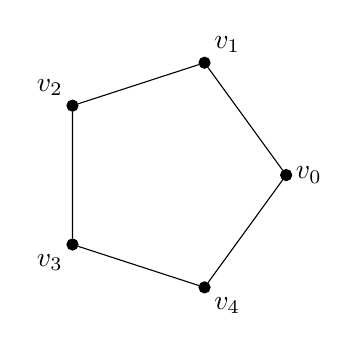
\begin{tikzpicture}[
  vtx/.style={
    circle, draw, fill=black,
    inner sep=0pt, minimum width=4pt
  }
]
  \foreach \ang/\x in {0/v0,72/v1,144/v2,216/v3,288/v4} {
    \node[vtx] (\x) at (\ang:1.5){};
  }
  \node[right] at (v0){$v_0$};
  \node[above right] at (v1){$v_1$};
  \node[above left] at (v2){$v_2$};
  \node[below left] at (v3){$v_3$};
  \node[below right] at (v4){$v_4$};
  \draw (v0)--(v1)--(v2)--(v3)--(v4)--(v0);
\end{tikzpicture}
\begin{tikzpicture}[
  vtx/.style={
    circle, draw, fill=black,
    inner sep=0pt, minimum width=4pt
  }
]
  \foreach \ang/\x in {0/v0,72/v1,144/v2,216/v3,288/v4} {
    \node[vtx] (\x) at (\ang:1.5){};
  }
  \node[right] at (v0){$v_1$};
  \node[above right] at (v1){$v_2$};
  \node[above left] at (v2){$v_3$};
  \node[below left] at (v3){$v_4$};
  \node[below right] at (v4){$v_0$};
  \draw (v0)--(v1)--(v2)--(v3)--(v4)--(v0);
  \draw[->] (-3,0)--(-2,0){} node[midway, above]{$s$};
  \node at (-3.25,0){};
\end{tikzpicture}
\begin{tikzpicture}[
  vtx/.style={
    circle, draw, fill=black,
    inner sep=0pt, minimum width=4pt
  }
]
  \foreach \ang/\x in {0/v0,72/v1,144/v2,216/v3,288/v4} {
    \node[vtx] (\x) at (\ang:1.5){};
  }
  \node[right] at (v0){$v_2$};
  \node[above right] at (v1){$v_3$};
  \node[above left] at (v2){$v_4$};
  \node[below left] at (v3){$v_0$};
  \node[below right] at (v4){$v_1$};
  \draw (v0)--(v1)--(v2)--(v3)--(v4)--(v0);
  \draw[->] (-3,0)--(-2,0){} node[midway, above]{$s$};
  \node at (-3.25,0){};
\end{tikzpicture}

\begin{tikzpicture}[
  vtx/.style={
    circle, draw, fill=black,
    inner sep=0pt, minimum width=4pt
  }
]
  \foreach \ang/\x in {0/v0,72/v1,144/v2,216/v3,288/v4} {
    \node[vtx] (\x) at (\ang:1.5){};
  }
  \node[right] at (v0){$v_3$};
  \node[above right] at (v1){$v_4$};
  \node[above left] at (v2){$v_0$};
  \node[below left] at (v3){$v_1$};
  \node[below right] at (v4){$v_2$};
  \draw (v0)--(v1)--(v2)--(v3)--(v4)--(v0);
  \draw[->] (-3,0)--(-2,0){} node[midway, above]{$s$};
\end{tikzpicture}
\begin{tikzpicture}[
  vtx/.style={
    circle, draw, fill=black,
    inner sep=0pt, minimum width=4pt
  }
]
  \foreach \ang/\x in {0/v0,72/v1,144/v2,216/v3,288/v4} {
    \node[vtx] (\x) at (\ang:1.5){};
  }
  \node[right] at (v0){$v_4$};
  \node[above right] at (v1){$v_0$};
  \node[above left] at (v2){$v_1$};
  \node[below left] at (v3){$v_2$};
  \node[below right] at (v4){$v_3$};
  \draw (v0)--(v1)--(v2)--(v3)--(v4)--(v0);
  \draw[->] (-3,0)--(-2,0){} node[midway, above]{$s$};
  \node at (-3.25,0){};
\end{tikzpicture}
\begin{tikzpicture}[
  vtx/.style={
    circle, draw, fill=black,
    inner sep=0pt, minimum width=4pt
  }
]
  \foreach \ang/\x in {0/v0,72/v1,144/v2,216/v3,288/v4} {
    \node[vtx] (\x) at (\ang:1.5){};
  }
  \node[right] at (v0){$v_0$};
  \node[above right] at (v1){$v_1$};
  \node[above left] at (v2){$v_2$};
  \node[below left] at (v3){$v_3$};
  \node[below right] at (v4){$v_4$};
  \draw (v0)--(v1)--(v2)--(v3)--(v4)--(v0);
  \draw[->] (-3,0)--(-2,0){} node[midway, above]{$s$};
  \node at (-3.25,0){};
\end{tikzpicture}

Let $r$ be reflection through the $x$-axis.

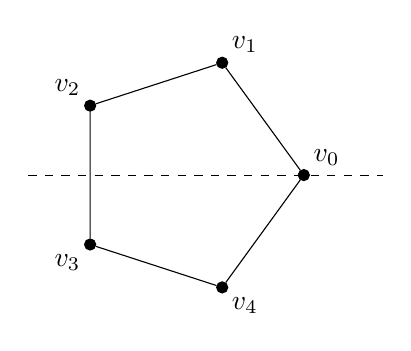
\begin{tikzpicture}[
  vtx/.style={
    circle, draw, fill=black,
    inner sep=0pt, minimum width=4pt
  }
]
  \foreach \ang/\x in {0/v0,72/v1,144/v2,216/v3,288/v4} {
    \node[vtx] (\x) at (\ang:1.5){};
  }
  \node[above right] at (v0){$v_0$};
  \node[above right] at (v1){$v_1$};
  \node[above left] at (v2){$v_2$};
  \node[below left] at (v3){$v_3$};
  \node[below right] at (v4){$v_4$};
  \draw (v0)--(v1)--(v2)--(v3)--(v4)--(v0);
  \draw[dashed] (-2,0)--(2.5,0);
\end{tikzpicture}
\begin{tikzpicture}[
  vtx/.style={
    circle, draw, fill=black,
    inner sep=0pt, minimum width=4pt
  }
]
  \foreach \ang/\x in {0/v0,72/v1,144/v2,216/v3,288/v4} {
    \node[vtx] (\x) at (\ang:1.5){};
  }
  \node[above right] at (v0){$v_0$};
  \node[above right] at (v1){$v_4$};
  \node[above left] at (v2){$v_3$};
  \node[below left] at (v3){$v_2$};
  \node[below right] at (v4){$v_1$};
  \draw (v0)--(v1)--(v2)--(v3)--(v4)--(v0);
  \draw[->] (-3,0)--(-2,0) node[midway, above]{$r$};
  \node at (-3.25,0){};
\end{tikzpicture}

$\abs{r} = 2$, that is, $r^2 = e$ and $r \neq e$.

We have $r(v_0) = v_0$ and $r(v_1)$ is now the vertex before $v_0$ rather than the vertex after.

\pagebreak
\subsection{Putting rotation and reflection together}

$s^i$ for $0 \leq i < n$ sends $v_0 \mapsto v_i$ and $v_1 \mapsto v_{i + 1}$.
(Say $v_n = v_0$ and $s^0 = e$.)

$s^i r$ for $0 \leq i < n$ sends $v_0 \mapsto v_i$ and $v_1 \mapsto v_{i - 1}$.
(Say $v_{-1} = v_{n - 1}$.)

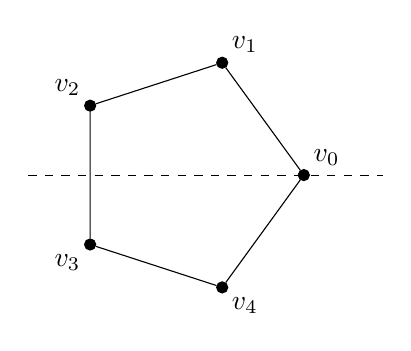
\begin{tikzpicture}[
  vtx/.style={
    circle, draw, fill=black,
    inner sep=0pt, minimum width=4pt
  }
]
  \foreach \ang/\x in {0/v0,72/v1,144/v2,216/v3,288/v4} {
    \node[vtx] (\x) at (\ang:1.5){};
  }
  \node[above right] at (v0){$v_0$};
  \node[above right] at (v1){$v_1$};
  \node[above left] at (v2){$v_2$};
  \node[below left] at (v3){$v_3$};
  \node[below right] at (v4){$v_4$};
  \draw (v0)--(v1)--(v2)--(v3)--(v4)--(v0);
  \draw[dashed] (-2,0)--(2.5,0);
\end{tikzpicture}
\begin{tikzpicture}[
  vtx/.style={
    circle, draw, fill=black,
    inner sep=0pt, minimum width=4pt
  }
]
  \foreach \ang/\x in {0/v0,72/v1,144/v2,216/v3,288/v4} {
    \node[vtx] (\x) at (\ang:1.5){};
  }
  \node[above right] at (v0){$v_0$};
  \node[above right] at (v1){$v_4$};
  \node[above left] at (v2){$v_3$};
  \node[below left] at (v3){$v_2$};
  \node[below right] at (v4){$v_1$};
  \draw (v0)--(v1)--(v2)--(v3)--(v4)--(v0);
  \draw[->] (-3,0)--(-2,0) node[midway, above]{$r$};
  \node at (-3.25,0){};
\end{tikzpicture}
\begin{tikzpicture}[
  vtx/.style={
    circle, draw, fill=black,
    inner sep=0pt, minimum width=4pt
  }
]
  \foreach \ang/\x in {0/v0,72/v1,144/v2,216/v3,288/v4} {
    \node[vtx] (\x) at (\ang:1.5){};
  }
  \node[above right] at (v0){$v_2$};
  \node[above right] at (v1){$v_1$};
  \node[above left] at (v2){$v_0$};
  \node[below left] at (v3){$v_4$};
  \node[below right] at (v4){$v_3$};
  \draw (v0)--(v1)--(v2)--(v3)--(v4)--(v0);
  \draw[->] (-3,0)--(-2,0) node[midway, above]{$s^2$};
  \node at (-3.25,0){};
\end{tikzpicture}

\begin{prop}{}{}
  $D_{2n} = \{ s^i r^j : 0 \leq i < n, \ 0 \leq j < 2 \}$, so $\abs{D_{2n}} = 2n$.
\end{prop}

So what is $rs$?

$rs(v_0) = r(v_1) = v_{n - 1}$ and $rs(v_1) = r(v_2) = v_{n - 2}$.

So $rs = s^{n - 1} r = s^{-1} r$.

\begin{cor}{}{}
  $D_{2n}$ is a finite non-abelian group.
\end{cor}

In summary:
\begin{itemize}
  \item $D_{2n} = \{ s^i r^j : 0 \leq i < n, \ 0 \leq j < 2 \}$
  \item $\abs{D_{2n}} = 2n$
  \item $s^n = e$, $r^2 = e$, $rs = s^{-1} r$
  \item $D_{2n}$ is a finite non-abelian group.
\end{itemize}
Exercise: show these relations are enough to completely determine $D_{2n}$.

\pagebreak
\subsection{What's group theory about?}

Basic answer: sets with one binary operation.

Better answer: group theory is the study of symmetry.

If we resize or rotate $P_n$, then the symmetries remain the same.

Kleinian view of geometry:
\begin{itemize}
  \item $D_{2n}$ captures what is means to be a regular $n$-gon.
  \item More generally, geometry is about the study of symmetries.
\end{itemize}

\pagebreak
\subsection{Permutation groups}

If $X$ is a set, let $\Fun(X, X)$ be the set of functions $X \to X$.
Then
\[ \circ \colon \Fun(X, X) \times \Fun(X, X) \to \Fun(X, X) : (f, g) \mapsto f \circ g \]
is an associative operation with an identity $\Id_X$.

Let $S_X = \{ f \in \Fun(X, X) : f \text{ is a bijection} \}$.

\begin{prop}{}{}
  $S_X$ is a group under $\circ$.
\end{prop}

\begin{thmproof}
  Homework.
\end{thmproof}

\begin{defn}{symmetric group}{symmetricgroup}
  Let $n \geq 1$.
  The \hldef{symmetric group} (or \hldef{permutation group}) $S_n$ is the group $S_X$ with
  $X = \{1, \ldots, n\}$.
\end{defn}

Elements of $S_n$ are bijections $\pi \colon \{1, \ldots, n\} \to \{1, \ldots, n\}$.

What makes such a $\pi$ a bijection?
Every element of $\{1, \ldots, n\}$ must appear in the list $\pi(1), \ldots, \pi(n)$ and no
element can appear twice.

We have $n$ choices for $\pi(1)$, $n - 1$ choices for $\pi(2)$, \dots, 1 choice for $\pi(n)$.
Thus $\abs{S_n} = n(n - 1) \cdots 1 = n!$.

Note $\abs{S_1} = 1! = 1$, so $S_1$ is the trivial group.

\pagebreak
\subsection{Permutations}

Elements of $S_n$ are called \hldef{permutations}.
We have several ways of representing permutations:
\begin{enumerate}
  \item
  Two-line representation:
  \[ \pi = \begin{pmatrix} 1 & 2 & 3 & 4 & 5 & 6 \\ 6 & 5 & 1 & 4 & 2 & 3 \end{pmatrix} \]
  \item
  One-line representation: $\pi = 651423$.
  \item
  Disjoint cycle representation: write down the \hldef{cycles} of $\pi$.
  Here $\pi(1) = 6$, $\pi(6) = 3$, and $\pi(3) = 1$, so $(163)$ is a cycle of $\pi$.

  $\pi = (163)(25)(4) = (163)(25)$.
  We typically drop cycles of length 1, and write cycles containing the smallest unused element
  first.

  The identity is empty in disjoint cycle notation, so we just use $e$.
\end{enumerate}

Multiplication can be done in two-line or disjoint cycle notation:
\begin{align*}
  \pi &= \begin{pmatrix}
    1 & 2 & 3 & 4 & 5 & 6 \\
    6 & 5 & 1 & 4 & 2 & 3
  \end{pmatrix} = (163)(25) \\
  \sigma &= \begin{pmatrix}
    1 & 2 & 3 & 4 & 5 & 6 \\
    2 & 6 & 4 & 5 & 3 & 1
  \end{pmatrix} = (126)(345) \\
  \pi\sigma &= \begin{pmatrix}
    1 & 2 & 3 & 4 & 5 & 6 \\
    5 & 3 & 4 & 2 & 1 & 6
  \end{pmatrix} = (15)(234)
\end{align*}
One-line notation is hard, so we don't use it here.

Inversion can also be done in two-line or disjoint cycle notation:
\[
  \pi = \begin{pmatrix}
    1 & 2 & 3 & 4 & 5 & 6 \\
    6 & 5 & 1 & 4 & 2 & 3
  \end{pmatrix} = (163)(25)
\]
\[
  \pi^{-1} = \begin{pmatrix}
    6 & 5 & 1 & 4 & 2 & 3 \\
    1 & 2 & 3 & 4 & 5 & 6
  \end{pmatrix} = \begin{pmatrix}
    1 & 2 & 3 & 4 & 5 & 6 \\
    3 & 5 & 6 & 4 & 2 & 1
  \end{pmatrix} = (136)(25)
\]
If $\pi(i) = j$, then $\pi^{-1}(j) = i$, so cycles of $\pi^{-1}$ are cycles of $\pi$ in reverse
order.

\pagebreak
\subsection{Fixed points and support sets}

\begin{defn}{fixed point, support set}{fixedpoint_supportset}
  The \hldef{fixed points} of a permutation $\pi \in S_n$ are the numbers $1 \leq i \leq n$ such
  that $\pi(i) = i$.

  The \hldef{support set} of $\pi \in S_n$ is
  \[ \supp(\pi) = \{ 1 \leq i \leq n : \pi(i) \neq i \}. \]

  $\pi$ and $\sigma$ are \hldef{disjoint} if $\supp(\pi) \cap \supp(\sigma) = \varnothing$.
\end{defn}

\begin{ex}
  $\supp((163)(25)) = \{1, 2, 3, 5, 6\}$.
\end{ex}

Some notes:
\begin{itemize}
  \item
  In general, $\supp(\pi)$ are exactly the numbers that appear in the disjoint cycle representation
  of $\pi$ (when length-1 cycles are omitted).
  \item
  $\supp(\pi) = \varnothing$ if and only if $\pi = e$.
  \item
  $\supp(\pi^{-1}) = \supp(\pi)$.
  \item
  If $i \in \supp(\pi)$, then $\pi(i) \in \supp(\pi)$.
\end{itemize}

\pagebreak
\subsection{Commuting elements}

\begin{defn}{commute}{commute}
  Two elements $g, h$ in a group $G$ \hldef{commute} if $gh = hg$.
\end{defn}

\begin{lem}{}{}
  If $\pi, \sigma \in S_n$ are disjoint, then $\pi\sigma = \sigma\pi$.
\end{lem}

\begin{thmproof}
  Suppose $1 \leq i \leq n$.

  If $i \in \supp(\pi)$, then $\pi(i) \in \supp(\pi)$.
  Since $\pi, \sigma$ are disjoint, we have $i, \pi(i) \not\in \supp(\sigma)$.
  So $\pi(\sigma(i)) = \pi(i) = \sigma(\pi(i))$.

  By symmetry, $\pi(\sigma(i)) = \sigma(\pi(i))$ if $i \in \supp(\sigma)$.

  If $i \not\in \supp(\pi) \cup \supp(\sigma)$, then $\pi(\sigma(i)) = i = \sigma(\pi(i))$.

  Then $\pi(\sigma(i)) = \sigma(\pi(i))$ for all $i$, so $\pi\sigma = \sigma\pi$.
\end{thmproof}

\pagebreak
\subsection{Cycles}

\begin{defn}{cycle}{cycle}
  A \hldef{$k$-cycle} is an element of $S_n$ with disjoint cycle notation $(i_1 i_2 \cdots i_k)$.
\end{defn}

Suppose the cycles of $\pi \in S_n$ are $c_1, \ldots, c_k$.
We can regard $c_i$ as an element of $S_n$ and $\pi = c_1 \cdot c_2 \cdot \cdots \cdot c_k$ as a
product in $S_n$.
Since $c_i$ and $c_j$ are disjoint, $c_i c_j = c_j c_i$.
Thus the order of cycles in disjoint cycle representation doesn't matter.

\begin{ex}
  $\pi = (163)(25) = (25) \cdot (163)$.
\end{ex}

Additionally, we have $\pi^{-1} = c_k^{-1} \cdots c_1^{-1} = c_1^{-1} \cdots c_k^{-1}$.

\begin{ex}
  If $c$ and $c'$ are non-disjoint cycles, then they don't necessarily commute:
  $(12)(23) = (123)$ while $(23)(12) = (123)^{-1} = (132) \neq (12)(23)$.
\end{ex}

If $\pi$ is a permutation, then $\pi$ commutes with $\pi^i$ for all $i$, so $\pi$ and $\pi^i$
commute.
However, $\pi$ and $\pi^i$ don't have disjoint support sets.

%---------------
\end{document}
%---------------
